\section{Step-by-Step Implementation Manuals}
\label{sec:manuals}

Rubric Section~IV (\qty{50}{\percent} of the total evaluation) mandates four reproducible operational manuals accompanied by complete institutional source code in Appendices~\ref{app:unillanos_html}--\ref{app:pki_scripts}. To avoid duplication with the member inventory in Rubric Section~I, this section details Manual~1 (\qty{10}{\percent}: ZeroTier SD-WAN provisioning, static IP pinning, and MTU/MSS tuning) and Manual~2 (\qty{10}{\percent}: multi-tenant HTTPS/HTTP server engineering, OS persistence, and intranet UI walkthrough), while the companion PKI trust and authoritative DNS manuals (Manuals~3 and~4, \qty{15}{\percent} each) follow in the next section.

\subsection{Manual 1 (10\%): ZeroTier SD-WAN Network Creation and Configuration}
\label{subsec:manual1_sdwan}

ZeroTier decouples its cryptographic control plane (Virtual Layer~1, VL1) from a flat virtual Ethernet switching fabric (Virtual Layer~2, VL2), encapsulating Ethernet frames inside encrypted UDP port~9993 tunnels across heterogeneous NAT and ISP boundaries~\cite{zerotier2024,tanenbaum2021,kurose2017}. Provisioning the bilateral COIL overlay proceeds through five deterministic stages.

\subsubsection{Network Creation and Private Access Control}
Log in to ZeroTier Central (\nolinkurl{https://my.zerotier.com}) and click \textbf{Create A Network} to allocate a globally unique 64-bit (16-hexadecimal-character) Network ID, assigned to this project as \texttt{abfd31bd47affa39}. Under \textbf{Settings} $\rightarrow$ \textbf{Basics}, enter the descriptive network name \textit{COIL Group 2 SD-WAN - UniLlanos \& Seneca} and set \textbf{Access Control} to \textbf{Private}. Enforcing \textit{Private} admission ensures that the controller drops VL2 traffic from any 40-bit ZeroTier Node ID whose cryptographic identity has not been explicitly authorized~\cite{zerotier2024}.

\subsubsection{Managed Routing, IPv4/IPv6 Pools, Multicast, and DNS Push}
Under \textbf{Settings} $\rightarrow$ \textbf{Advanced}, define the IPv4 addressing plan and link-layer controls shown in Fig.~\ref{fig:zerotier_settings}:
\begin{itemize}
    \item \textbf{Managed Routes:} Add \nolinkurl{172.22.0.0/16} with a blank \texttt{Via} field (marking it as an on-link \texttt{LAN} route) so every authorized member routes inter-institutional traffic directly across the virtual switch without an external gateway hop.
    \item \textbf{IPv4 Auto-Assign:} Enable \textbf{Easy} mode and select the \nolinkurl{172.22.*.*} block (\nolinkurl{172.22.0.1}--\nolinkurl{172.22.255.254}), isolating the SD-WAN from overlapping residential \nolinkurl{192.168.x.x} and campus \nolinkurl{10.x.x.x} subnets.
    \item \textbf{Multicast \& Broadcast Policy:} Set \textbf{Multicast Recipient Limit} to \num{32} and check \textbf{Enable Broadcast}, guaranteeing standard ARP discovery within \nolinkurl{172.22.0.0/16} while bounding WAN multicast replication overhead.
\end{itemize}

\begin{figure*}[t]
\centering
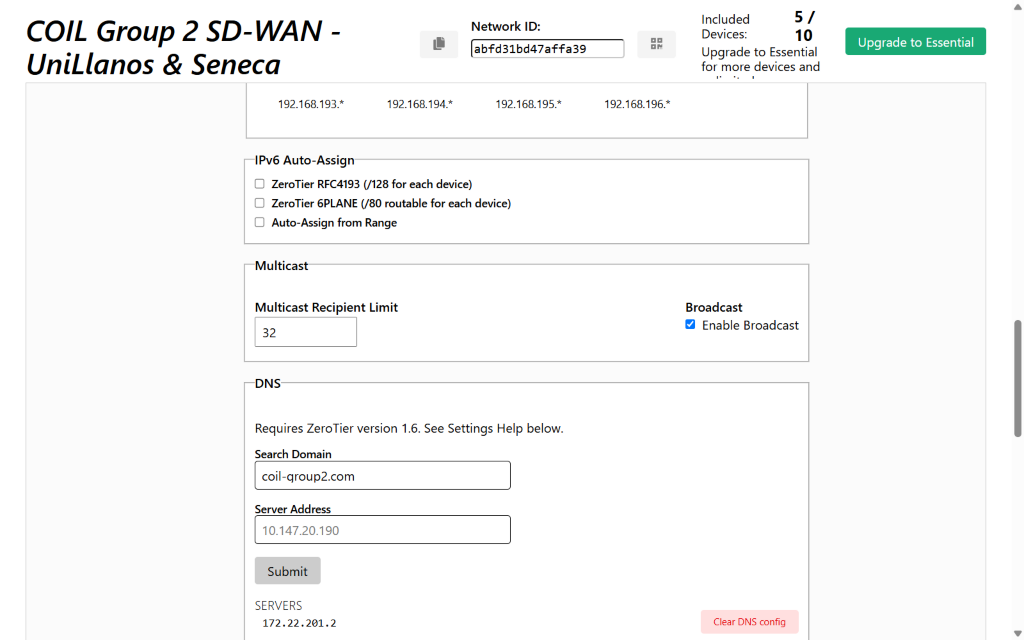
\includegraphics[width=0.84\textwidth]{figuras/zerotier_settings_dns_fresh.png}
\caption{ZeroTier Central advanced configuration console for Network ID \texttt{abfd31bd47affa39}, illustrating the IPv4 Easy Auto-Assign grid edge, disabled IPv6 auto-assignment checkboxes, Multicast Recipient Limit (\num{32}) with Broadcast enabled, and the ZeroTier~1.6+ authoritative DNS push configuration (\texttt{coil-group2.com} served by \texttt{172.22.201.2}).}
\label{fig:zerotier_settings}
\end{figure*}

As captured in Fig.~\ref{fig:zerotier_settings}, every panel in the ZeroTier Central settings view plays an explicit engineering role:
\begin{enumerate}
    \item \textbf{Top Network Header:} Displays the title \textit{COIL Group 2 SD-WAN - UniLlanos \& Seneca}, clipboard and QR-code enrollment shortcuts for \texttt{abfd31bd47affa39}, the free-tier quota counter (\textit{Included Devices: 5 / 10}), and the plan upgrade banner.
    \item \textbf{IPv4 Auto-Assign Grid:} Only the bottom row (\nolinkurl{192.168.193.*}--\nolinkurl{192.168.196.*}) falls within the scrolled viewport edge, above which the active \nolinkurl{172.22.*.*} subnet allocation is selected.
    \item \textbf{IPv6 Auto-Assign Panel:} All three checkboxes---\textit{ZeroTier RFC4193 (/128 for each device)}, \textit{ZeroTier 6PLANE (/80 routable for each device)}, and \textit{Auto-Assign from Range}---remain intentionally unchecked so Windows and Android hosts keep IPv4-only SD-WAN routing, eliminating extraneous ICMPv6 neighbor discovery and \texttt{AAAA} DNS queries in packet captures.
    \item \textbf{Multicast Panel:} Displays \textbf{Multicast Recipient Limit} fixed at \num{32} alongside the checked \textbf{Broadcast} (\textit{Enable Broadcast}) box.
    \item \textbf{DNS Panel:} Indicates the \textit{Requires ZeroTier version 1.6} prerequisite, specifies \textbf{Search Domain} as \nolinkurl{coil-group2.com}, displays the \textbf{Server Address} input field (placeholder \nolinkurl{10.147.20.190}) and \textbf{Submit} button, and confirms \nolinkurl{172.22.201.2} under \textbf{SERVERS} (with a \textbf{Clear DNS config} reset control) to push authoritative DNS automatically to enrolled nodes (detailed further in Manual~4).
\end{enumerate}

\subsubsection{Client Installation and Elevated Network Enrollment}
Deploy the ZeroTier One client across all five institutional and student endpoints---Miguel's UniLlanos web server laptop, the simulated Seneca gateway (\texttt{miguel2}), Luis Alejandro's Windows workstation, and both Android smartphones:
\begin{enumerate}
    \item \textbf{Windows Desktop and Server Nodes (\texttt{v1.16.2}):} Install the \texttt{x86\_64} ZeroTier One service silently from PowerShell using \texttt{winget}, as shown in Listing~\ref{lst:zt_join}.
    \item \textbf{Android Mobile Nodes (\texttt{v1.16.0}):} Install ZeroTier One (\texttt{arm64}) from Google Play, tap \textbf{Add Network}, and enroll \texttt{abfd31bd47affa39} (or scan the header QR code).
    \item \textbf{Elevated Windows CLI Join:} On Windows, the local ZeroTier daemon secures its IPC token (\texttt{C:\textbackslash{}ProgramData\textbackslash{}\allowbreak ZeroTier\textbackslash{}One\textbackslash{}\allowbreak authtoken.secret}) with Administrator-only permissions; non-elevated terminals exit with an unreadable-token error. Open an elevated Administrator PowerShell session and execute Listing~\ref{lst:zt_join} on each Windows host.
\end{enumerate}

\begin{lstlisting}[caption={Windows ZeroTier One installation, elevated join, and MTU tuning commands.},label={lst:zt_join}]
# 1. Install ZeroTier One (v1.16.2 x86_64) via winget
winget install zerotier.zerotierone --silent `
  --accept-package-agreements --accept-source-agreements

# 2. Join SD-WAN from elevated Administrator PowerShell
zerotier-cli join abfd31bd47affa39
zerotier-cli listnetworks

# 3. Clamp virtual interface MTU to 1300 B (MSS = 1260 B)
Set-NetIPInterface `
  -InterfaceAlias "ZeroTier One [abfd31bd47affa39]" `
  -AddressFamily IPv4 -NlMtuBytes 1300
netsh interface ipv4 show subinterfaces
\end{lstlisting}

\subsubsection{Device Authorization, Role Labeling, and Static IP Pinning}
In the ZeroTier Central \textbf{Members} table, verify each incoming Node ID against its local \texttt{zerotier-cli info} output, check the \textbf{Auth} box, and enforce the rubric's descriptive \textit{Name + Website} naming convention so evaluators can immediately distinguish servers from student clients. Pin static virtual IPv4 addresses by removing ephemeral dynamic leases and assigning deterministic addresses within \nolinkurl{172.22.0.0/16}: \nolinkurl{172.22.201.2} for the UniLlanos web/DNS server, \nolinkurl{172.22.31.69} for the Seneca partner gateway, and \nolinkurl{172.22.100.11} for Luis Alejandro's Windows workstation (complemented by Android client leases). Rather than duplicating the complete five-node registry here, Table~\ref{tab:zerotier_members} and Fig.~\ref{fig:sdwan_topology} in Rubric Section~I provide the authoritative member inventory, firmware versions (\texttt{v1.16.2} on Windows and \texttt{v1.16.0} on Android), physical endpoints, and mesh topology.

\subsubsection{Interface MTU Tuning for Fragmentation-Free Transport}
ZeroTier's default virtual Ethernet MTU of \qty{2800}{\byte} exceeds standard physical Ethernet (\qty{1500}{\byte}), PPPoE DSL (\qty{1492}{\byte}), and mobile cellular LTE/5G bearer MTUs (\qtyrange{1400}{1420}{\byte}) once VL1 UDP/cryptographic encapsulation headers are prepended~\cite{zerotier2024,tanenbaum2021}. Left untuned, large TLS certificate chains trigger outer-UDP fragmentation and packet loss across strict cellular NATs. Executing \texttt{Set-NetIPInterface} in Listing~\ref{lst:zt_join} constrains the ZeroTier virtual adapter to an IPv4 MTU of \qty{1300}{\byte}, verified via \texttt{netsh} on both the UniLlanos host and the Seneca gateway. Subtracting the mandatory \qty{20}{\byte} IPv4 header and \qty{20}{\byte} standard TCP header yields an exact Maximum Segment Size of $\text{MSS} = 1300 - 40 = \qty{1260}{\byte}$, matching the TCP three-way handshake negotiation observed in Rubric Section~III's Wireshark trace.

\subsection{Manual 2 (10\%): Multi-Tenant Web Server Creation and Intranet UI Deployment}
\label{subsec:manual2_web}

Both institutions must host cultural intranets accessible by IPv4 address and domain URL over TLS-encrypted HTTPS. Rather than relying on separate web engines, COIL Group~2 implemented a lightweight, zero-dependency threaded Python server (\texttt{COIL-DualIntranet/2.0}) paired with three dark-themed HTML5/CSS3 portals.

\subsubsection{Repository Directory Hierarchy and Dual-Node Deployment}
All server code, PKI credentials, DNS scripts, and static web assets are organized deterministically beneath \nolinkurl{modulo2/}, launched by \nolinkurl{iniciar_pagina.bat} (\qty{4445}{\byte}) at the repository root:
\begin{itemize}
    \item \nolinkurl{certificados/}: Private Root CA (\nolinkurl{COIL_Group2_Root_CA.crt}), OpenSSL SAN policy (\nolinkurl{openssl.cnf}), leaf key (\nolinkurl{server-key.pem}), and certificate chain (\nolinkurl{fullchain.pem}).
    \item \nolinkurl{dns/}: Authoritative \texttt{dnslib} daemon (\nolinkurl{dns_server.py}) and hosts fallback helper (\nolinkurl{setup_hosts.ps1}).
    \item \nolinkurl{servidor/}: Multi-tenant server engine (\nolinkurl{server_https.py}, reproduced in Appendix~\ref{app:server_https}).
    \item \nolinkurl{sitio_web/}: Segregated document roots for \nolinkurl{portal/} (\nolinkurl{index.html}, \qty{6941}{\byte}), \nolinkurl{unillanos/} (\nolinkurl{index.html}, \qty{18520}{\byte}, plus 12 regional images in \nolinkurl{img/}), and \nolinkurl{seneca/} (\nolinkurl{index.html}, \qty{15470}{\byte}, plus 7 Canadian assets in \nolinkurl{img/}).
\end{itemize}
On the UniLlanos node (\nolinkurl{172.22.201.2}), the stack runs directly from the primary repository directory. To maintain symmetric institutional availability on the partner node (\texttt{miguel2}, \nolinkurl{172.22.31.69}), the identical \nolinkurl{certificados/}, \nolinkurl{dns/}, \nolinkurl{servidor/}, and \nolinkurl{sitio_web/} hierarchy is synchronized to \texttt{C:\textbackslash{}COIL\_Server\textbackslash{}} with runtime output logged to \texttt{C:\textbackslash{}COIL\_Server\textbackslash{}server.log}.

\subsubsection{Multi-Tenant Server Engine Architecture}
As detailed in Listing~\ref{lst:server_https}, \nolinkurl{server_https.py} combines two custom classes built on Python's standard library:

\textit{Non-Blocking Threaded TLS Wrapper:} Standard \texttt{http.server.ThreadingHTTPServer} implementations that invoke \texttt{ssl\_context.wrap\_socket()} inside \texttt{get\_request()} execute the TLS handshake synchronously on the main listener thread, allowing a stalled or scanning peer to freeze the entire server. To eliminate head-of-line blocking, \texttt{NonBlockingSSLThreadingServer} inherits from \texttt{socketserver.ThreadingMixIn} and \texttt{http.server.HTTPServer} with \texttt{daemon\_threads = True} and \texttt{request\_queue\_size = 32}. It overrides \texttt{process\_request\_thread(self, request, client\_address)} to move TLS negotiation into each worker thread:
\begin{enumerate}
    \item Applies \texttt{request.settimeout(10.0)} (\qty{10.0}{\second}) prior to \texttt{self.ssl\_context.\allowbreak wrap\_socket(\allowbreak request, server\_side=True)} so incomplete ClientHello probes abort cleanly.
    \item Sets \texttt{ssl\_sock.settimeout(15.0)} (\qty{15.0}{\second}) on the encrypted socket before calling \texttt{finish\_request()}.
    \item Catches \texttt{ssl.SSLError}, \texttt{socket.timeout}, \texttt{ConnectionResetError}, and \texttt{BrokenPipeError} without crashing sibling threads, closing the active socket inside a guaranteed \texttt{finally} block.
\end{enumerate}

\textit{Dual-Protocol Binding and TLS~1.3 Context:} A daemon background thread executes \texttt{socketserver.\allowbreak ThreadingTCPServer(\allowbreak("0.0.0.0", 80), \allowbreak DualIntranetHandler)} for fallback HTTP access, while the main thread binds \texttt{0.0.0.0:443} using \texttt{ssl.SSLContext(ssl.PROTOCOL\_TLS\_SERVER)}, loading \nolinkurl{fullchain.pem} and \nolinkurl{server-key.pem} and advertising ALPN \texttt{["http/1.1"]}. (The module also provides \texttt{HTTPRedirectHandler} with a \qty{10}{\second} timeout issuing HTTP~\texttt{301} redirects to \texttt{https://\{host\}\{path\}} when strict redirect-only port~80 enforcement is desired.)

\textit{Virtual-Host Routing, Hardening, and RFC~9110 Headers:} \texttt{DualIntranetHandler} (\texttt{server\_version = "COIL-DualIntranet/2.0"}, \texttt{protocol\_version = "HTTP/1.1"}, \texttt{timeout = 15}) supports both \texttt{do\_GET()} and \texttt{do\_HEAD()} (`head\_only=True`). Table~\ref{tab:server_routes} summarizes the routing rules, MIME handling, and security headers emitted per RFC~9110~\cite{rfc9110}.

\begin{table}[t]
\centering
\caption{Request Routing, Security Guard, and HTTP/1.1 Header Policy in \texttt{COIL-DualIntranet/2.0}}
\label{tab:server_routes}
\footnotesize
\setlength{\tabcolsep}{4pt}
\renewcommand{\arraystretch}{1.2}
\begin{tabularx}{\columnwidth}{@{} >{\raggedright\arraybackslash}p{2.95cm} >{\raggedright\arraybackslash}X @{}}
\toprule
\textbf{Mechanism / Route} & \textbf{Server Behavior \& Emitted Headers} \\
\midrule
Host-based routing & Strips port from \texttt{Host}; prefixes \nolinkurl{/unillanos} for \texttt{unillanos.*} and \nolinkurl{/seneca} for \texttt{seneca.*}. \\
\addlinespace[2pt]
Portal \& tenant paths & \nolinkurl{/} or \nolinkurl{/index.html} $\rightarrow$ \nolinkurl{portal/index.html}; \nolinkurl{/unillanos/} and \nolinkurl{/seneca/} map to institutional roots. \\
\addlinespace[2pt]
Canonical 301 & \nolinkurl{/unillanos} $\rightarrow$ \texttt{301} \nolinkurl{/unillanos/}; \nolinkurl{/seneca} $\rightarrow$ \texttt{301} \nolinkurl{/seneca/}. \\
\addlinespace[2pt]
Root CA & \nolinkurl{/ca.crt} or \nolinkurl{/COIL_Group2_Root_CA.crt} serves \nolinkurl{COIL_Group2_Root_CA.crt} as \texttt{application/x-x509-ca-cert} attachment. \\
\addlinespace[2pt]
Traversal guard & \texttt{os.path.normpath()} checks prefix against \texttt{SITIO\_DIR}; returns HTTP~\texttt{403} on escape attempts, \texttt{404} if absent. \\
\addlinespace[2pt]
MIME \& security & Explicit \texttt{.webp}/\texttt{.avif} mapping; emits \texttt{Connection: close}, \texttt{Cache-Control: no-cache}, \texttt{X-Content-Type-Options: nosniff}, and conditional \texttt{Strict-Transport-Security: max-age=0} on \texttt{SSLSocket}. \\
\bottomrule
\end{tabularx}
\end{table}

\subsubsection{Firewall Provisioning, Automated Launcher, and Scheduled Task Persistence}
Three host-level configurations guarantee uninterrupted access across Windows Defender Firewall and headless reboots:
\begin{enumerate}
    \item \textbf{Windows Firewall Rules:} Create inbound TCP allow rules \texttt{COIL\_HTTPS\_443} (port~443) and \texttt{COIL\_HTTP\_80} (port~80) using \texttt{New-NetFirewallRule} (Listing~\ref{lst:win_deploy}) so ZeroTier overlay peers can establish TCP connections across Windows Private and Public network profiles.
    \item \textbf{Automated Batch Launcher (\texttt{iniciar\_pagina.bat}):} Accepts \texttt{--no-browser} and \texttt{--no-wait} arguments, locates Python~3, inspects \texttt{netstat -ano -p UDP} (`0.0.0.0:53`) and \texttt{dnslib} before starting \nolinkurl{dns_server.py}, checks TCP port~443 \texttt{LISTENING} status, launches \nolinkurl{server_https.py} with unbuffered output (\texttt{python -u}), polls up to \qty{8}{\second} for socket readiness, opens \nolinkurl{https://www.coil-group2.com/}, and exposes an interactive \texttt{[R/D/S]} console menu (\texttt{[R]} reopen browser, \texttt{[D]} terminate both Python daemons via WMI \texttt{Win32\_Process} filtering, \texttt{[S]} exit while keeping daemons running).
    \item \textbf{Headless Scheduled Task Persistence (\texttt{COIL\_HTTPS\_Daemon}):} On the Seneca gateway (\texttt{miguel2}, \texttt{C:\textbackslash{}COIL\_Server}), \texttt{COIL\_HTTPS\_Daemon} runs \texttt{python.exe -u C:\textbackslash{}COIL\_Server\textbackslash{}\allowbreak servidor\textbackslash{}server\_https.py} in \texttt{C:\textbackslash{}COIL\_Server} using an \texttt{S4U} (\textit{Interactive/Background}) logon principal. Because \texttt{DualIntranetHandler.log\_message()} and \texttt{process\_request\_thread()} invoke \texttt{sys.stderr.write()} and \texttt{sys.stderr.flush()}, launching the server with GUI-subsystem \texttt{pythonw.exe} leaves \texttt{sys.stderr} equal to \texttt{None} and raises an \texttt{AttributeError} on the first HTTP request or TLS error; pairing console \texttt{python.exe -u} with \texttt{S4U} persistence avoids any visible desktop console while preserving a valid \texttt{sys.stderr} handle.
\end{enumerate}

\begin{lstlisting}[caption={Windows Firewall rules and headless S4U Scheduled Task registration on the Seneca partner node.},label={lst:win_deploy}]
New-NetFirewallRule -DisplayName "COIL_HTTPS_443" `
  -Direction Inbound -Protocol TCP -LocalPort 443 -Action Allow
New-NetFirewallRule -DisplayName "COIL_HTTP_80" `
  -Direction Inbound -Protocol TCP -LocalPort 80 -Action Allow

$act = New-ScheduledTaskAction `
  -Execute "python.exe" `
  -Argument "-u C:\COIL_Server\servidor\server_https.py" `
  -WorkingDirectory "C:\COIL_Server"
$prin = New-ScheduledTaskPrincipal `
  -UserId $env:USERNAME -LogonType S4U
Register-ScheduledTask -TaskName "COIL_HTTPS_Daemon" `
  -Action $act -Principal $prin -Force
Start-ScheduledTask -TaskName "COIL_HTTPS_Daemon"
\end{lstlisting}

\subsubsection{Exhaustive Intranet User Interface (UI/GUI) Walkthrough}
The dual-intranet web suite comprises three standalone HTML5/CSS3 applications (Appendices~\ref{app:unillanos_html}--\ref{app:portal_html}) styled with a high-contrast dark slate palette, zero external JavaScript frameworks, and responsive CSS Grid layouts verified over HTTPS/TLS~1.3.

\begin{figure*}[t]
\centering
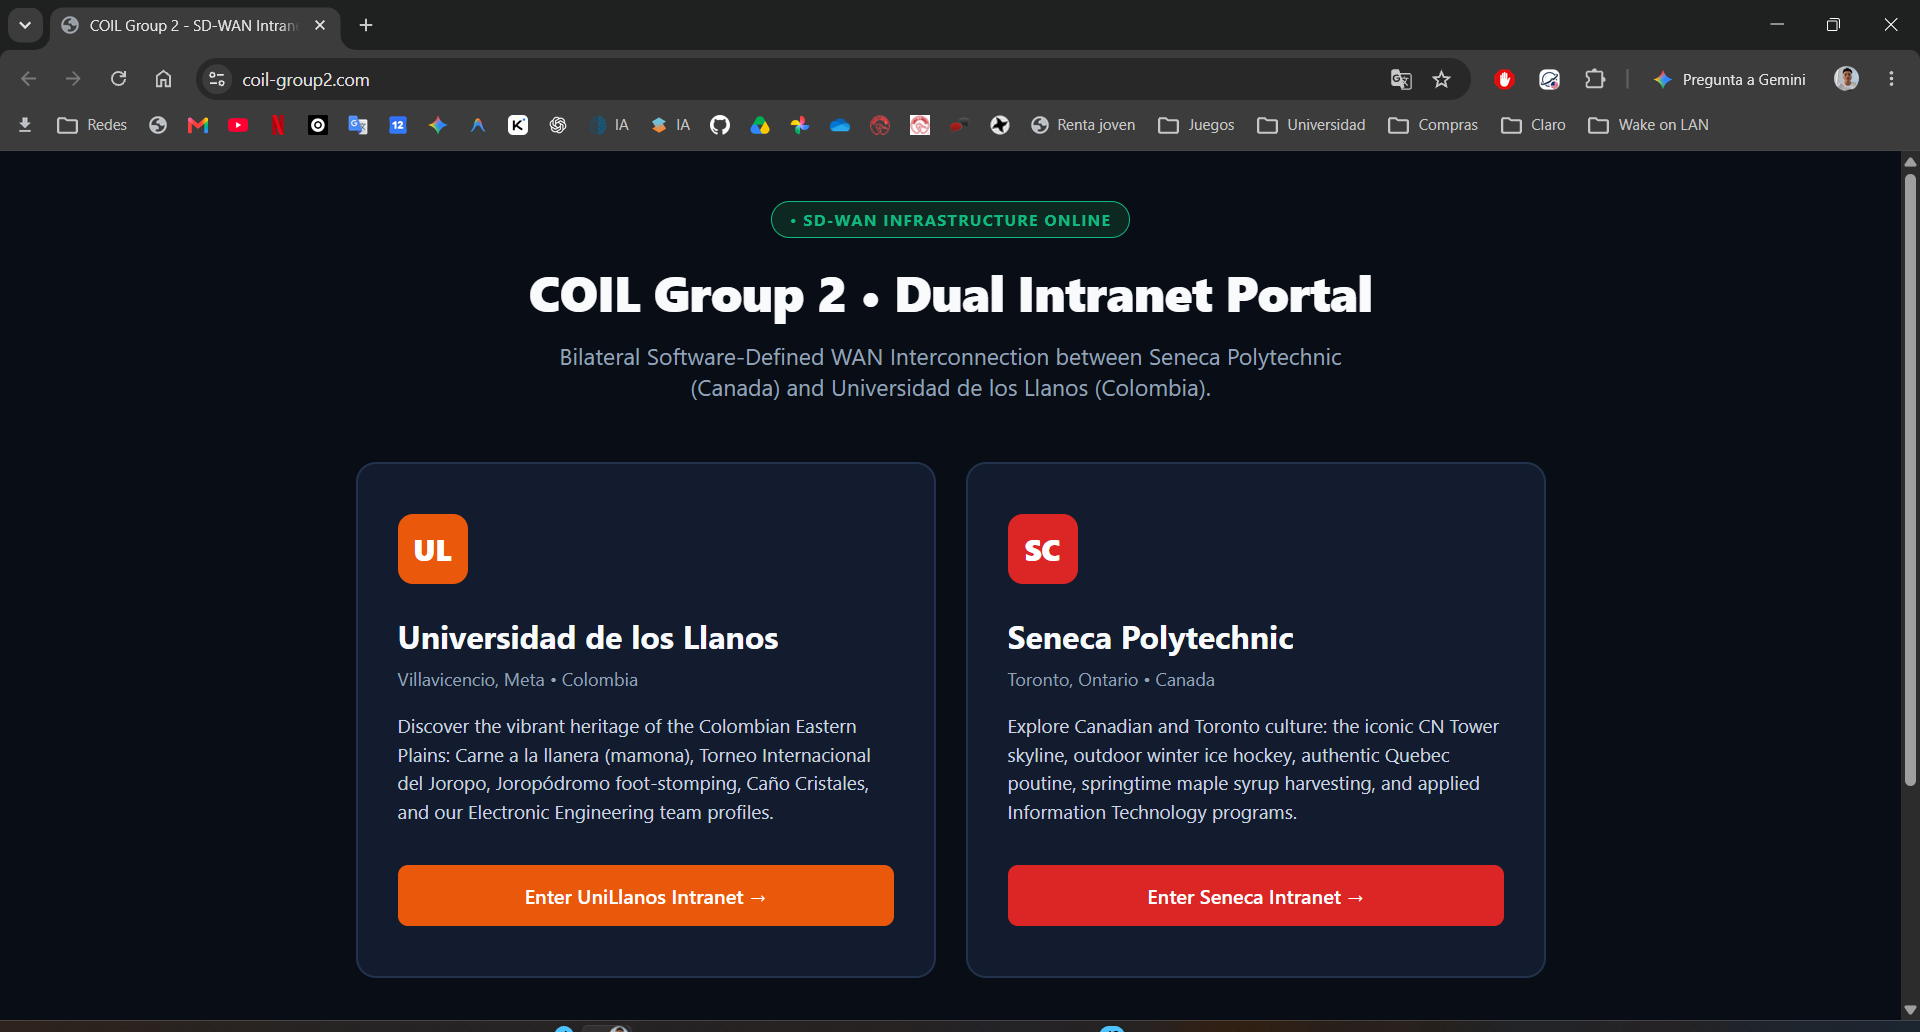
\includegraphics[width=0.90\textwidth]{figuras/ui_portal_fresh.png}
\caption{COIL Group~2 Dual Intranet Gateway Portal (\texttt{portal/index.html}, \qty{6941}{\byte}) rendered at \texttt{https://www.coil-group2.com/}, featuring the \textit{SD-WAN Infrastructure Online} badge, institutional \texttt{UL} and \texttt{SC} routing cards, and the bottom SD-WAN telemetry bar.}
\label{fig:ui_portal}
\end{figure*}

\textbf{1) Dual Intranet Gateway Portal (Fig.~\ref{fig:ui_portal}, Appendix~\ref{app:portal_html}):} Served at \nolinkurl{/} (\qty{6941}{\byte}), the gateway opens with an emerald status pill (\textit{SD-WAN Infrastructure Online}, \texttt{\#10b981}) above the bilateral title header. Its central CSS Grid (\texttt{repeat(auto-fit, minmax(300px, 1fr))}) presents two interactive institutional routing cards: \texttt{UL} (\textit{Universidad de los Llanos}, Villavicencio, Meta, styled with \texttt{\#ea580c} orange accents) and \texttt{SC} (\textit{Seneca Polytechnic}, Toronto, Ontario, styled with \texttt{\#dc2626} crimson accents), each applying a \texttt{translateY(-6px)} hover elevation and colored box-shadow transition. Below the cards, the telemetry status bar (\texttt{.network-bar}) displays four live infrastructure indicators: \textit{SD-WAN Mesh: ZeroTier Virtual Ethernet}, \textit{Host IP: 172.22.201.2}, \textit{Encryption: TLS 1.3 / HTTPS (Port 443)}, and \textit{Domain: www.coil-group2.com}. On narrow viewports, the \texttt{@media (max-width: 640px)} rule collapses \texttt{.gateways} to a single column (\texttt{1fr}) and stacks \texttt{.network-bar} items vertically.

\begin{figure*}[t]
\centering
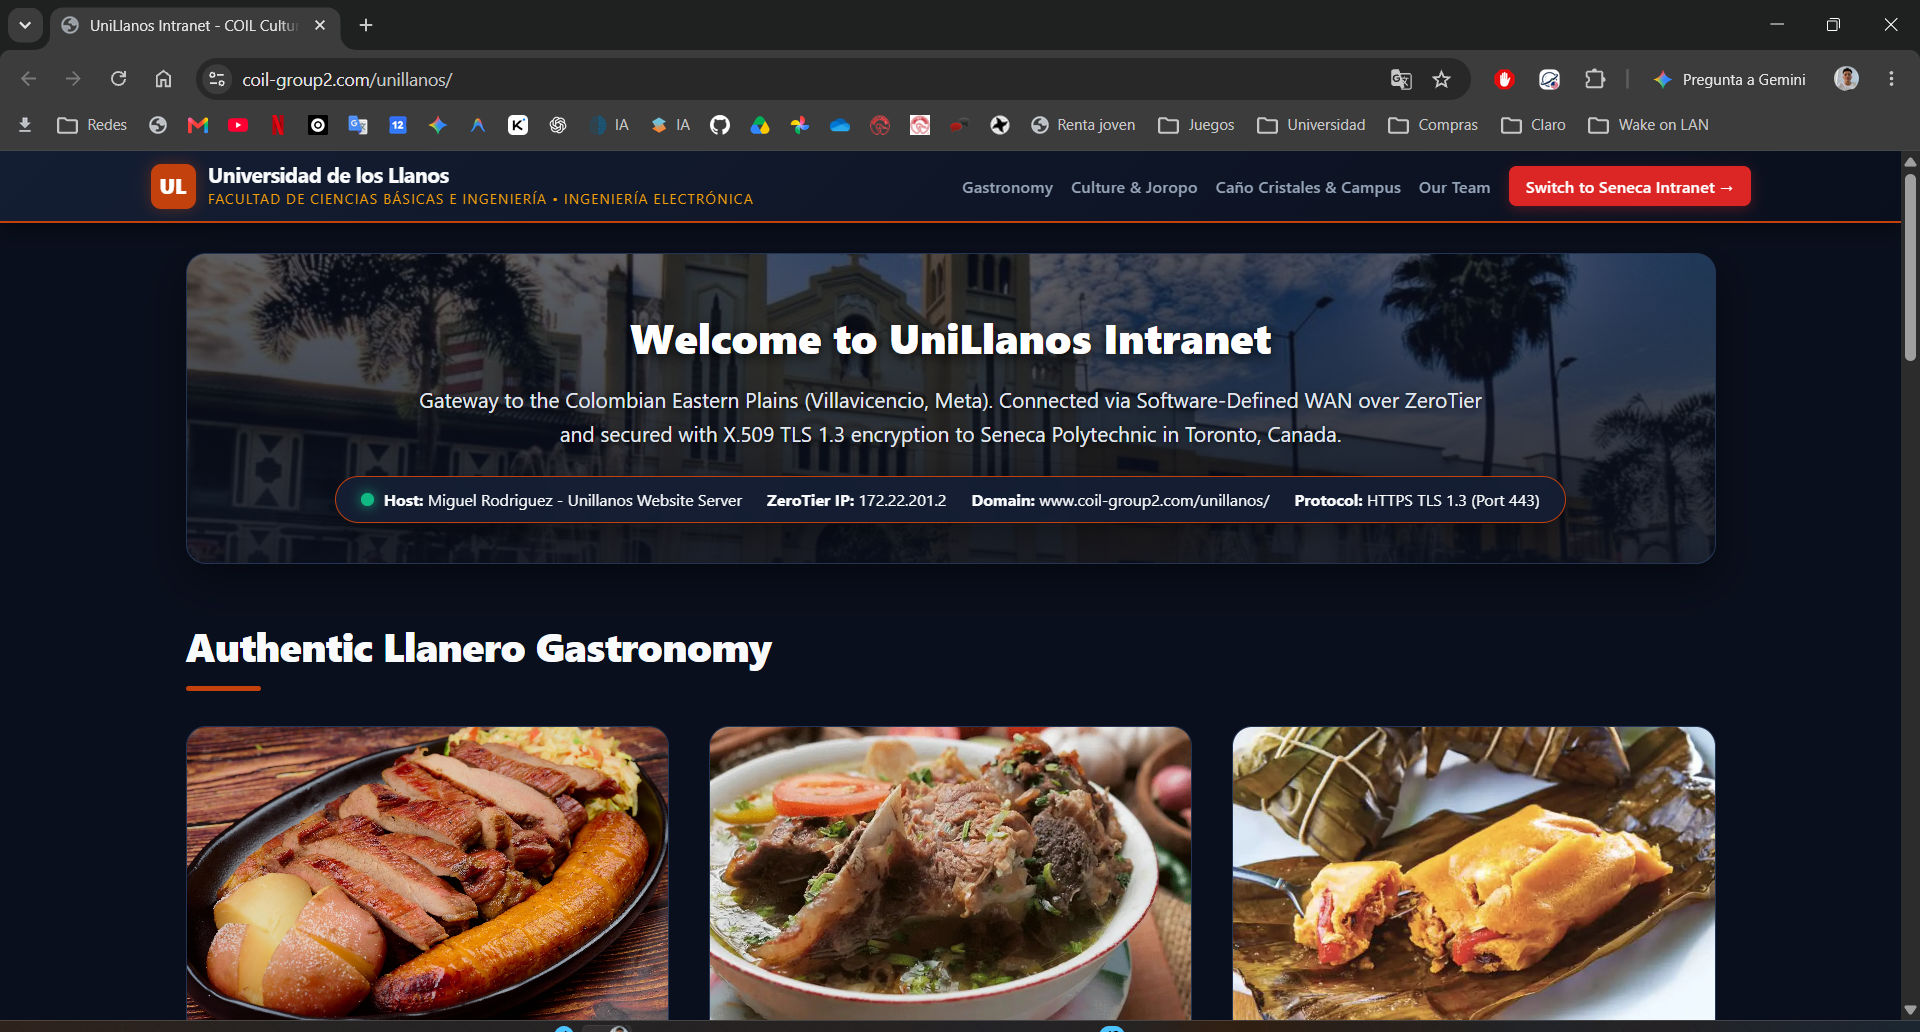
\includegraphics[width=0.90\textwidth]{figuras/ui_unillanos_fresh.png}
\caption{Universidad de los Llanos Cultural Intranet (\texttt{unillanos/index.html}, \qty{18520}{\byte}) rendered at \texttt{https://www.coil-group2.com/unillanos/}, showing the sticky \texttt{UL} navigation bar with the red \textit{Switch to Seneca Intranet} control, Villavicencio panorama hero with glassmorphism telemetry pill, Llanero cultural cards, and Engineering Team profiles.}
\label{fig:ui_unillanos}
\end{figure*}

\textbf{2) Universidad de los Llanos Intranet (Fig.~\ref{fig:ui_unillanos}, Appendix~\ref{app:unillanos_html}):} Served at \nolinkurl{/unillanos/} (\qty{18520}{\byte}), the Colombian portal features a sticky top navbar displaying the \texttt{UL} badge, faculty subtitle (\textit{Facultad de Ciencias B\'{a}sicas e Ingenier\'{i}a $\cdot$ Ingenier\'{i}a Electr\'{o}nica}), smooth anchor links (\texttt{\#gastronomy}, \texttt{\#festivals}, \texttt{\#nature}, \texttt{\#team}), and a prominent red (\texttt{\#dc2626}) \textit{Switch to Seneca Intranet} cross-routing button targeting \nolinkurl{/seneca/}. Its hero banner overlays \nolinkurl{img/villavicencio_panorama.jpg} with a glassmorphism telemetry pill (\texttt{backdrop-filter: blur(8px)}) embedding a glowing green status dot, \textit{Host: Miguel Rodriguez - Unillanos Website Server}, \textit{ZeroTier IP: 172.22.201.2}, \textit{Domain: www.coil-group2.com/unillanos/}, and \textit{Protocol: HTTPS TLS 1.3 (Port 443)}. Eight photographic cards with hover zoom (\texttt{scale(1.06)}) showcase Llanero gastronomy (\textit{Carne a la Llanera (Mamona)}, \textit{Caldo de Costilla}, \textit{Hayaca Llanera}), regional festivals and landscapes (\textit{Torneo del Joropo \& Jorop\'{o}dromo}, \textit{Sunsets of the Orinoco Basin}, \textit{Villavicencio Metropolis}), and natural heritage (\textit{Ca\~{n}o Cristales: River of Five Colors}, \textit{UniLlanos Barcelona Campus}). Below the grids, the \textit{UniLlanos Engineering Team} showcase presents circular avatar biographies for \textit{Miguel \'{A}ngel Rodr\'{i}guez Payares} (10th Semester, Electronic Engineering, lead server architect) and \textit{Luis Alejandro Le\'{o}n Vel\'{a}squez} (9th Semester, Electronic Engineering, English~C1). Under \texttt{@media (max-width: 768px)}, the navbar converts \texttt{.nav-links} into a touch-scrollable horizontal bar (\texttt{-webkit-overflow-scrolling: touch}), expands the partner button to full width, and centers team profiles vertically.

\begin{figure*}[t]
\centering
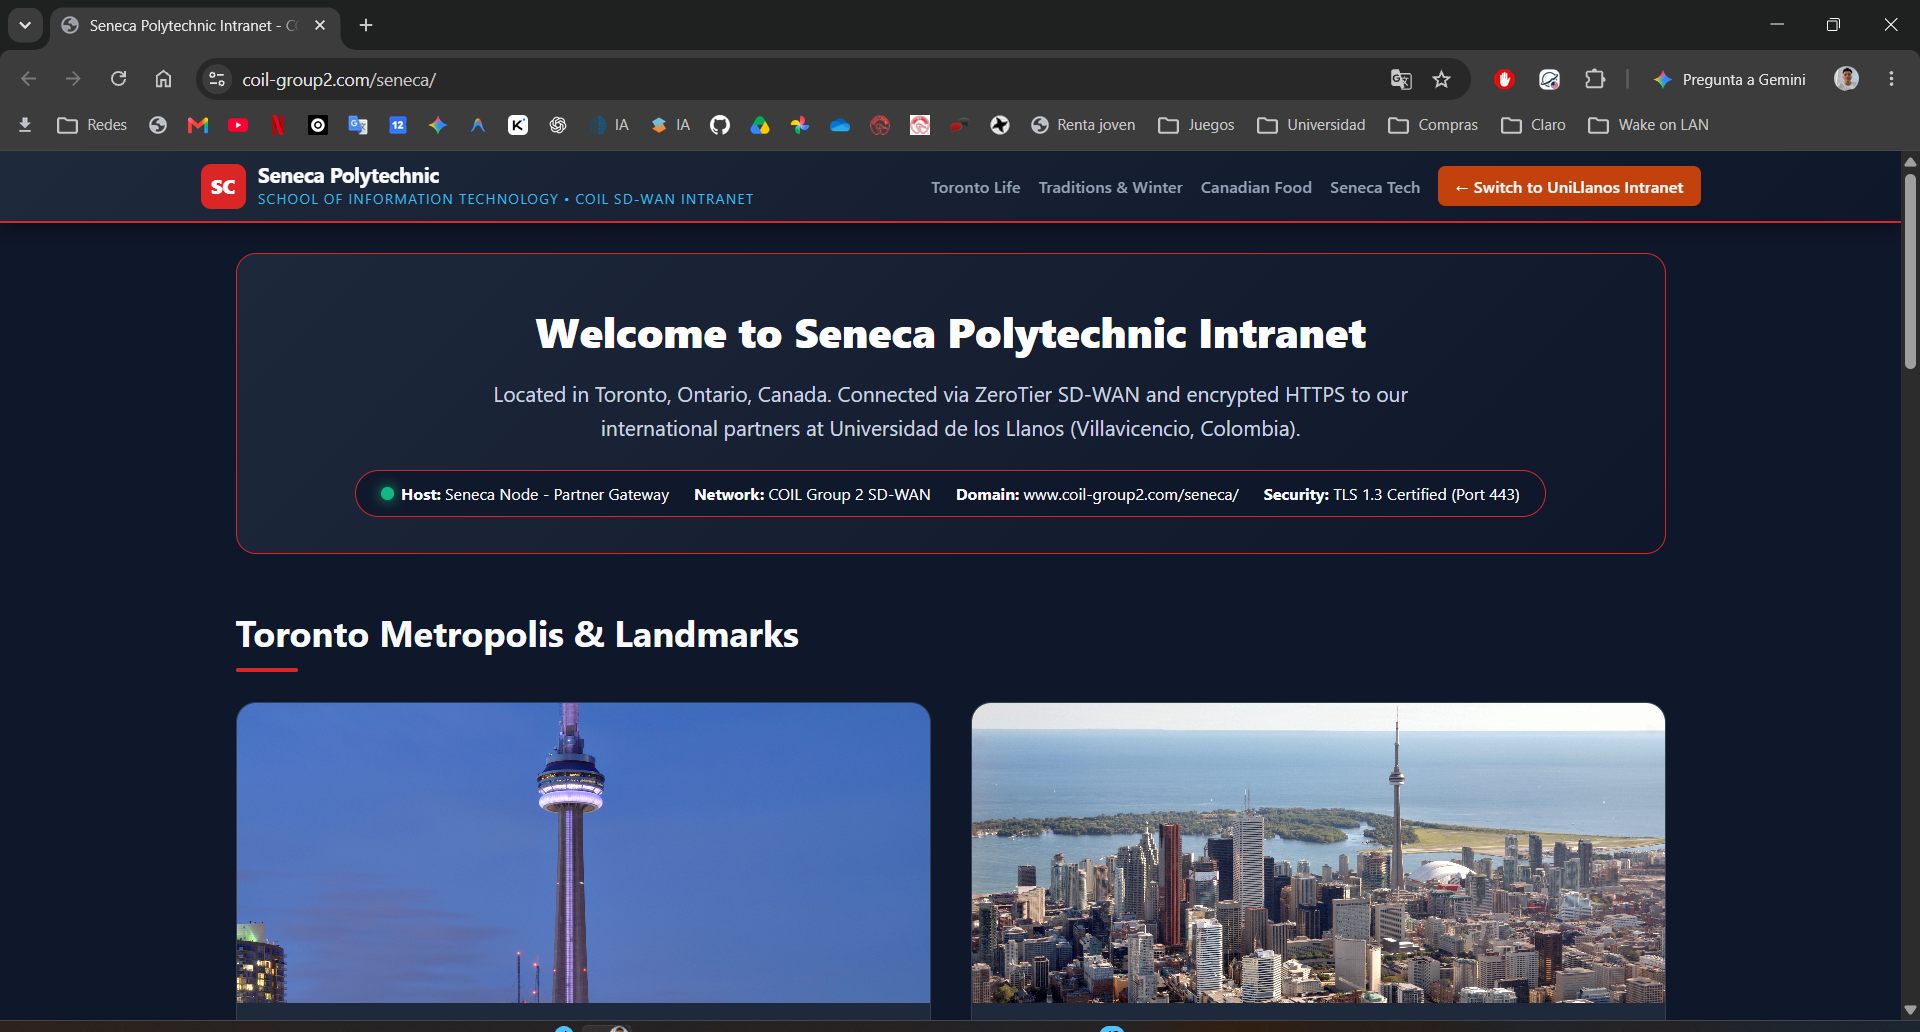
\includegraphics[width=0.90\textwidth]{figuras/ui_seneca_fresh.png}
\caption{Seneca Polytechnic Cultural Intranet (\texttt{seneca/index.html}, \qty{15470}{\byte}) rendered at \texttt{https://www.coil-group2.com/seneca/}, displaying the sticky \texttt{SC} header with the orange \textit{Switch to UniLlanos Intranet} return control, gateway telemetry pill, and Canadian cultural, culinary, and IT showcase cards.}
\label{fig:ui_seneca}
\end{figure*}

\textbf{3) Seneca Polytechnic Intranet (Fig.~\ref{fig:ui_seneca}, Appendix~\ref{app:seneca_html}):} Served at \nolinkurl{/seneca/} (\qty{15470}{\byte}), the Canadian partner portal mirrors the UniLlanos design system with crimson (\texttt{\#dc2626}) and sky-blue (\texttt{\#38bdf8}) accents. Its sticky header presents the \texttt{SC} badge, \textit{School of Information Technology $\cdot$ COIL SD-WAN Intranet} subheading, section anchors (\texttt{\#toronto}, \texttt{\#canadian-culture}, \texttt{\#gastronomy}, \texttt{\#academics}), and the reciprocal burnt-orange (\texttt{\#c2410c}) \textit{Switch to UniLlanos Intranet} button returning to \nolinkurl{/unillanos/}. The hero houses the partner telemetry pill (\textit{Host: Seneca Node - Partner Gateway}, \textit{Network: COIL Group 2 SD-WAN}, \textit{Domain: www.coil-group2.com/seneca/}, \textit{Security: TLS 1.3 Certified (Port 443)}), followed by eight lazy-loaded (\texttt{loading="lazy"}) cards across four domains: Toronto landmarks (\textit{CN Tower \& Downtown Skyline} at \qty{553.3}{\meter}, \textit{Lake Ontario \& Toronto Islands}), Canadian traditions (\textit{Ice Hockey \& Outdoor Rinks}, \textit{Maple Syrup \& Sugar Shacks}), culinary classics (\textit{Authentic Poutine}, \textit{Peameal Bacon \& Butter Tarts}), and bilateral academics (\textit{School of Information Technology}, \textit{UniLlanos $\cdot$ Seneca COIL Exchange}), sharing the identical \texttt{@media (max-width: 768px)} mobile touch layout.
